\documentclass[a4paper]{article}

\usepackage[italian]{babel}
\usepackage[utf8]{inputenc}
\usepackage{mathrsfs,amsmath}
\usepackage{graphicx}
\usepackage[colorinlistoftodos]{todonotes}
\usepackage{subfigure}
\usepackage{url}
\usepackage{xfrac}

\title{PIV image analysis}

\author{Claudio Caccia - 820091}

\date{\today}

\begin{document}
\maketitle

\begin{abstract}
Analisi di coppie di immagini PIV relative al campo di moto intorno ad un profilo alare di tipo NACA 23012. 
\end{abstract}

\section{Introduzione}
\label{sec:intro}

La \textit{Particle Image Velocimetry} (PIV) è un metodo per la visualizzazione qualitativa e quantitativa del campo di moto di un fluido mediante l'uso di particelle traccianti illuminate da una lama di luce e fotografate in due istanti successivi. I dati rilevanti per l'esperimento sono i seguenti:
\begin{itemize}
	\item profilo alare \textit{NACA 23012} di corda $30cm$,
	\item velocità galleria: $30m/s$,
	\item dimensione delle immagini: $1024 \times 1280$ pixel \textit{grayscale} (cfr. Figura \ref{fig:img}) 
	\item dimensione della finestra di analisi: $103\times82mm$
	\item intervallo tra i fotogrammi: $\Delta t = 10\mu s$
\end{itemize}

L'analisi si compone di tre fasi: \textit{preprocessing}, \textit{correlazione} ed \textit{analisi} dei risultati.

\section{Preprocessing}

Prima di procedere alla determinazione del campo di velocit\`{a} \`{e} opportuno analizzare le caratteristiche delle immagini ed eventualmente migliorarne la qualit\`{a}. Le tecniche di miglioramento possono riguardare:

\begin{itemize}
	\item \textit{Background subtraction}: tecnica utile ad eliminare lo sfondo comune alle immagini ed evidenziare solo il moto delle particelle. In genere serve una serie di immagini (almeno una decina) per poter eliminare lo sfondo in modo affidabile, pertanto non è stata impiegata qui.
	\item \textit{Filtraggio}:  varie tecniche utili a migliorare la distinzione tra particelle e sfondo e a ridurre il rumore di fondo.
\end{itemize}

Un utile passo preliminare consiste nell'analizzare la distribuzione dell'intensità di grigio dei pixel, come illustrato in Figura \ref{fig:hist}. Si evidenzia come sia presente una netta separazione, in entrambe le immagini, tra lo sfondo (maggioranza dei pixel scuri) e le particelle ad intensità massima.

\begin{figure}[h]
	\centering
	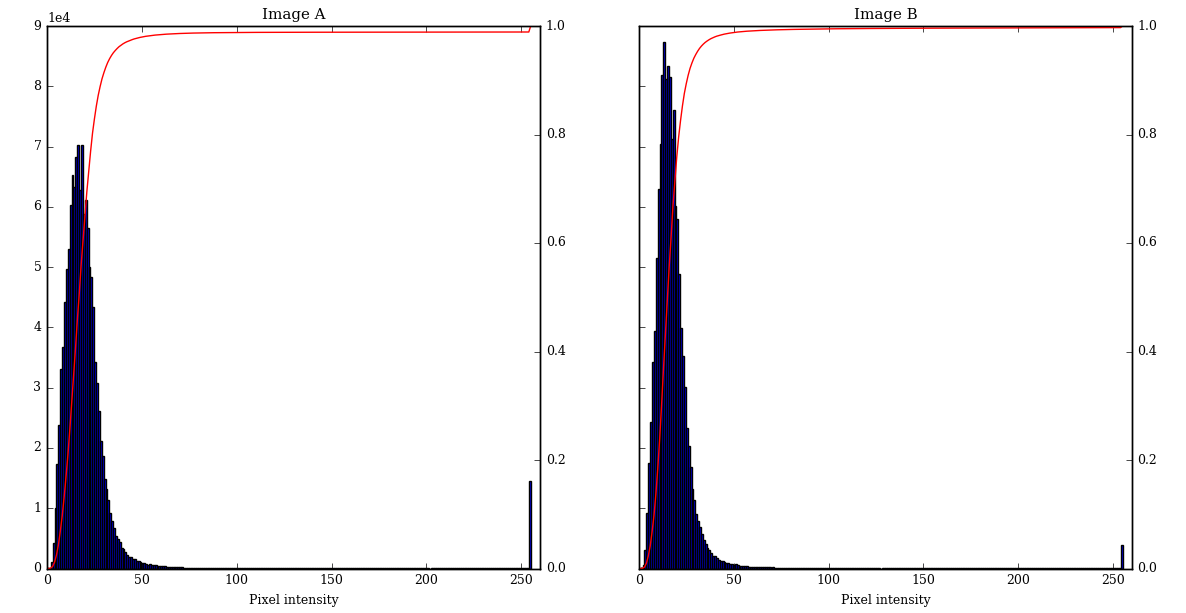
\includegraphics[width=1\textwidth]{images/hist_cr.png}
	\caption{\label{fig:hist}Istogrammi della distribuzione delle intensità di grigio}
\end{figure}

Per questo motivo si è deciso di utilizzare le immagini originali senza l'applicazione di filtri. Inoltre, alcune analisi preliminari hanno mostrato\footnote{Test effettuati utilizzando semplici filtri a soglia o di tipo \textit{min/max}\cite{mmaxf}} come l'utilizzo di immagini filtrate possa in questo caso produrre un maggior numero di correlazioni spurie rispetto alle immagini originali, a parità di condizioni di test (cfr. ad es. Figura \ref{fig:filt_piv} ).


\section{Algoritmo per PIV}
\label{sec:corr}

Il campo di velocità è ottenuto tramite \textit{correlazione} delle due immagini opportunamente traslate. I passi dell'algoritmo sono i seguenti:


\subsection{Definizione dell'algoritmo di correlazione}
Esistono diversi algoritmi \cite{corrCV} per effettuare la correlazione di due immagini. Sono stati considerati i seguenti:

\paragraph{Sum of Squared Differences [SSD]} Consiste in un algoritmo computazionalmente semplice, la miglior correlazione si trova nel punto di \textit{minimo} di:

\begin{equation}
R\left[x,y \right] = \sum_{i,j=-\sfrac{N}{2}}^{\sfrac{N}{2}} \left( A\left[i+x,j+y\right] - B\left[i,j \right] \right)^2
\label{eq:ssd}
\end{equation}

\paragraph{Normalized Cross Correlation [NCC]}\cite{imcorr},\cite{ncc}  Richiede il calcolo di media e deviazione standard delle immagini, la miglior correlazione si trova nel punto di \textit{massimo} di:

\begin{equation}
R\left[x,y \right] = \frac{ \sum_{i,j=-\sfrac{N}{2}}^{\sfrac{N}{2}} \left( A\left[i+x,j+y\right] - \mu_A \right) \cdot \left( B\left[i,j \right] - \mu_B \right) } { \sigma_A \cdot \sigma_B }
\label{eq:ncc}
\end{equation}


\paragraph{Discrete Fouries Transformation [DFT]} Richiede il calcolo delle trasformate delle immagini, la miglior correlazione si trova nel punto di \textit{massimo} di:

\begin{equation}
R = \mathscr{F}^{-1} \{ \mathscr{F}\{A\} \circ \mathscr{F}\{B\}^*    \}
\label{eq:dft}
\end{equation}

\subsection{Scelta delle finestre di interrogazione}

Trascurando aspetti computazionali, la dimensione delle finestre di interrogazione comporta un \textit{trade-off} tra una definizione accurata del campo di velocità, che richiede finestre di interrogazione piccole, e la bontà della correlazione, più affidabile con finestre grandi. I risultati più significativi sono stati ottenuti con finestre da \textbf{16} e \textbf{32} pixel.\\
Anche il massimo spostamento è un parametro da considerare: dai dati a disposizione, una velocità di $50 m/s$ corrisponde ad uno spostamento di circa $6.24px$ pertanto si considerano spostamenti massimi di \textbf{8} pixel. Le finestre di interrogazione sono pertanto:

\begin{equation}
I = \left[ 8+jN: 7+(j+1)N,8+kN: 7+(k+1)N\right] \quad N \in \{16,32 \} \quad j,k = 0 \ldots
\label{eq:int}
\end{equation}

\subsection{Interpolazione sub-pixel}

La correlazione definisce solamente spostamenti di pixel interi. Per raffinare il calcolo è possibile utilizzare algoritmi di interpolazione, come ad esempio descritto in \cite{spim}.

\paragraph{parabolic-fit estimator}

\begin{equation}
\epsilon =  \frac{R_{-1} - R_{+1} }{2\left( R_{-1} + R_{+1} -2 R_0   \right)}
\label{eq:pf}
\end{equation}



\paragraph{3 point gaussian-fit estimator}

\begin{equation}
\epsilon =  \frac{\ln(R_{-1}) - \ln(R_{+1}) }{2\left( \ln(R_{-1}) + \ln(R_{+1} -2 \ln(R_0)   \right)}
\label{eq:3pg}
\end{equation}

Le equazioni \ref{eq:pf} e \ref{eq:3pg} sono da applicare in entrambe le direzioni.\\
Nel caso di \textbf{NCC} è stato adottato l'algoritmo di \ref{eq:pf} in quanto immune a problemi di condizionamento legato ai logaritmi.
Nel caso di \textbf{DFT}, l'algoritmo adottato \cite{spdft} consente automaticamente di definire un livello di precisione \textit{sub-pixel}. 

\subsection{Fitting del profilo}

I dati geometrici a disposizione hanno permesso di effettuare il \textit{fitting} (manuale) del profilo alare rispetto alle immagini a disposizione. Questo ha consentito di comprendere meglio il campo di moto (soprattutto rispetto alla scala dimensionale del profilo) e di escludere tutte le correlazioni di elementi interni all'ala. Il fitting migliore è stato trovato a $7.2°$ di inclinazione rispetto all'asse della fotocamera ed è illustrato in figura \ref{fig:airfoil} dove si può anche visualizzare l'andamento della velocità.  


\section{Risultati}

Di seguito si riportano i principali risultati ottenuti dall'analisi PIV.

\subsection{SSD senza interpolazione sub-pixel}

Pur utilizzando una stima della correlazione semplice, si ottengono risultati interessanti, con pochi vettori di velocità palesemente spuri (cfr. figura \ref{fig:ssd}). L'unica zona difficile da correlare risulta essere la porzione visibile di intradosso, dove probabilmente vi è un afflusso non ottimale di particelle o il moto è particolarmente complesso. L'assenza di raffinamento \textit{sub-pixel} evidenzia un andamento della velocità costituito da regioni uniformi. Adottando una finestra a $16px$ comporta molti risultati spuri nello strato limite, come evidenziato in figura \ref{fig:ssd:a}.

\begin{figure}[h]
	\centering
	\subfigure[PIV con SSD - finestra 16px\label{fig:ssd:a}]
	{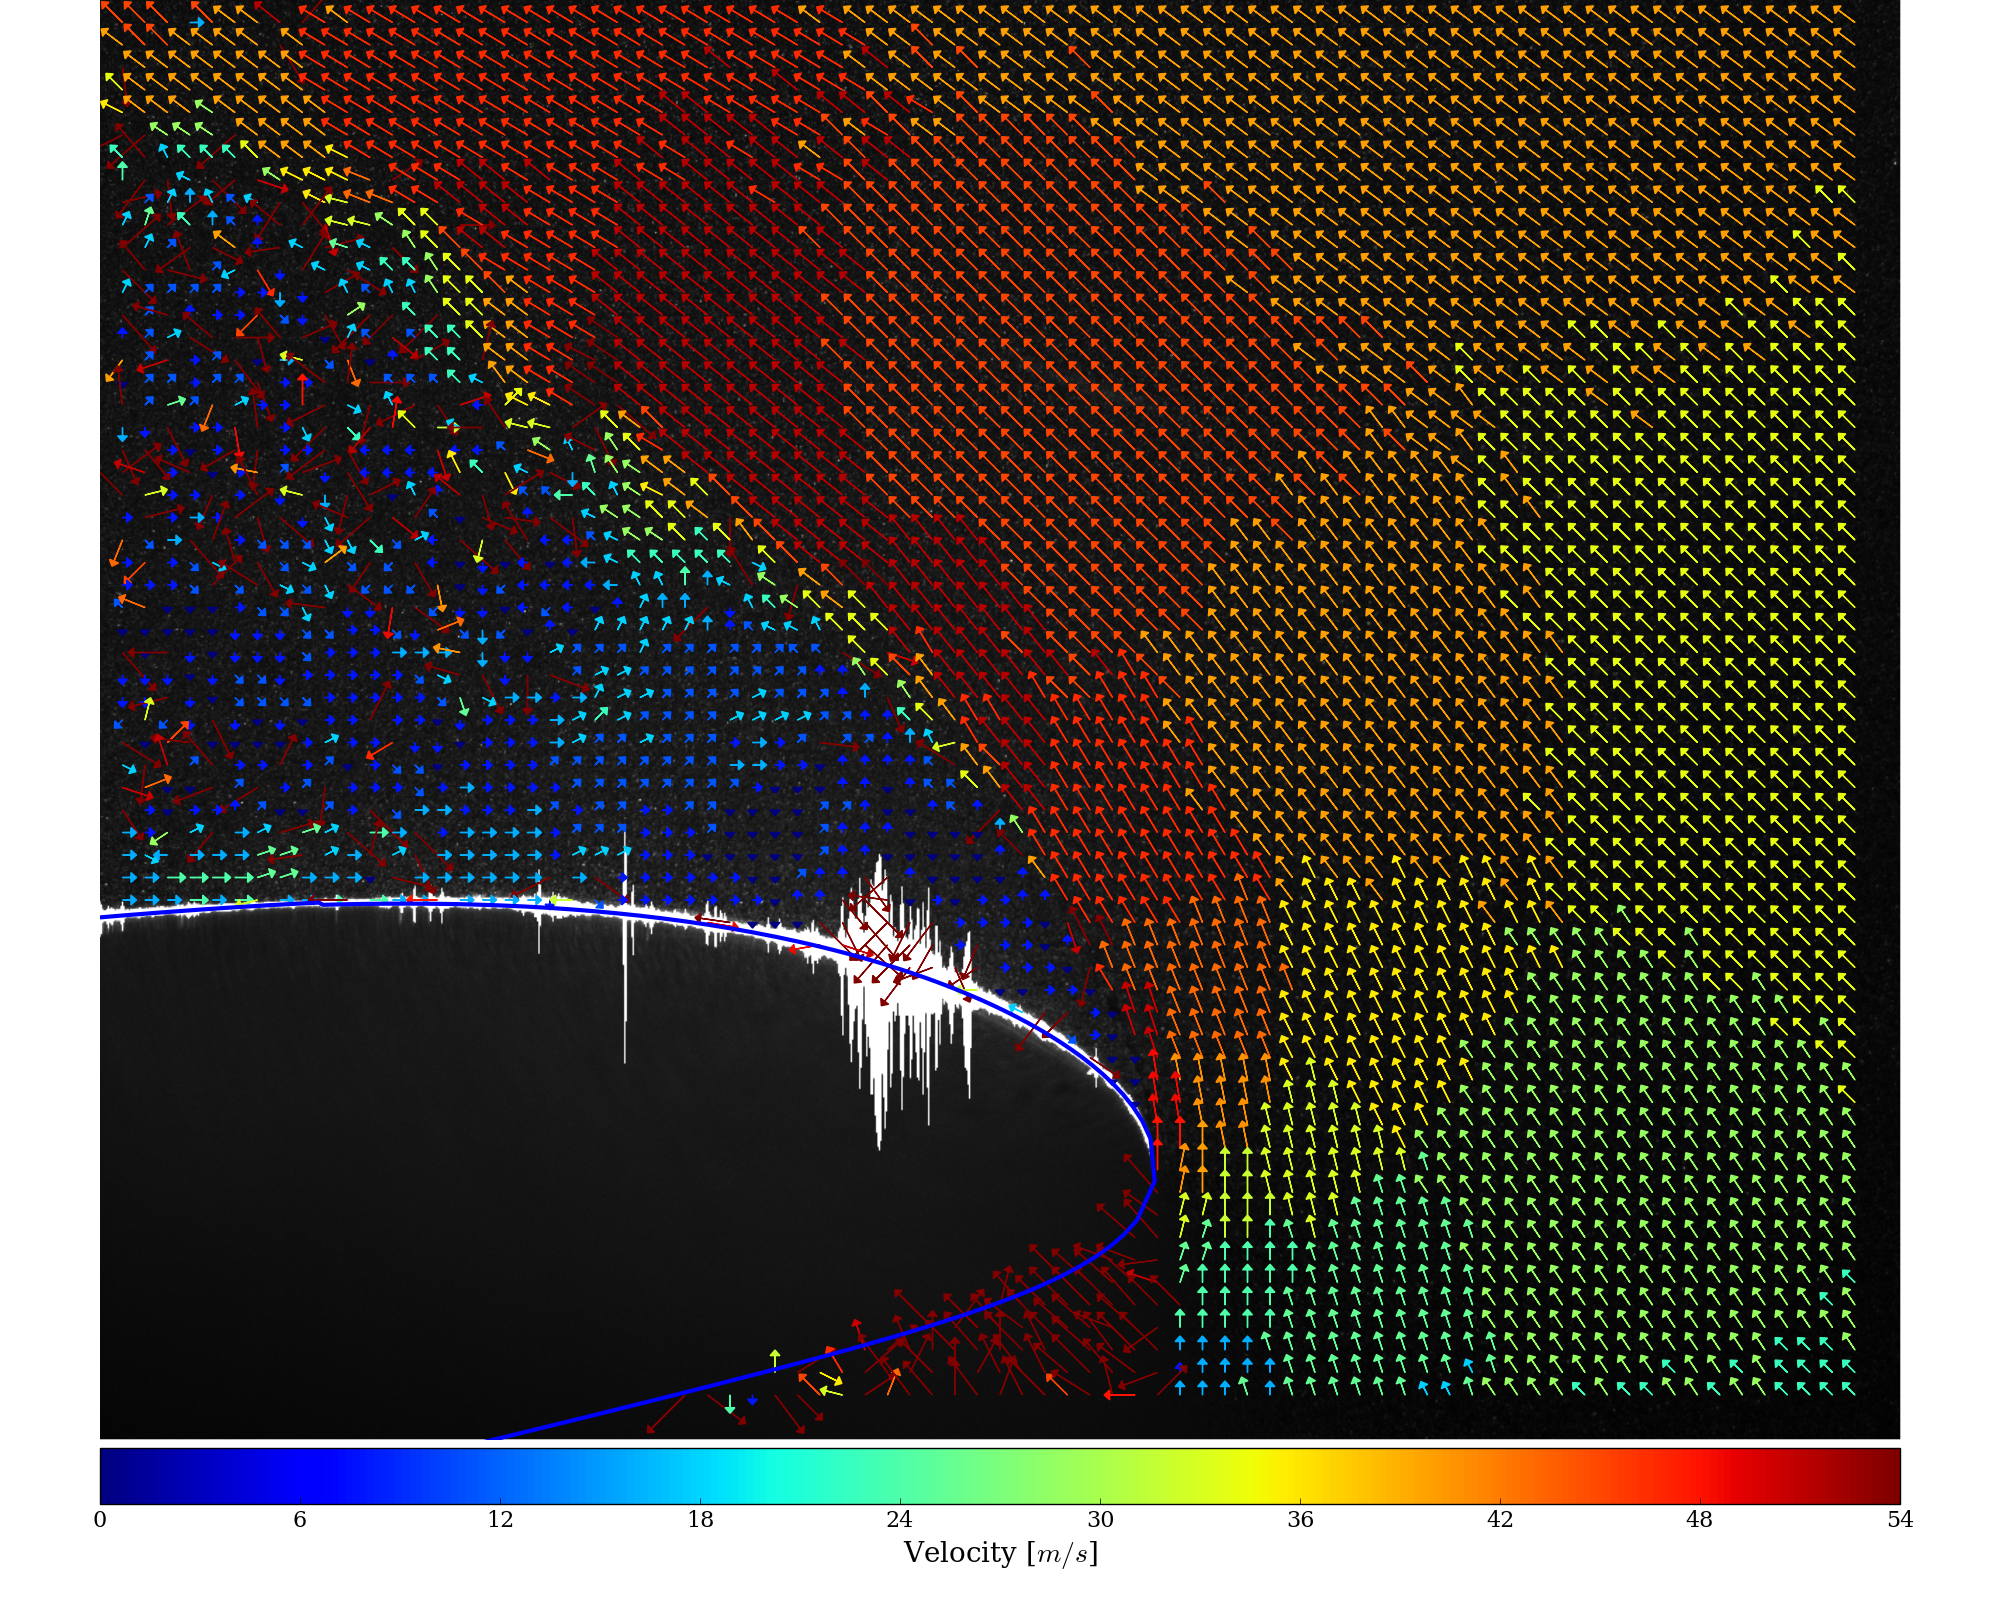
\includegraphics[width=0.48\textwidth]{images/ssd_CM_16_orig.png}}
	%\hspace{0.3\textwidth}
	\subfigure[PIV con SSD - finestra 32px\label{fig:ssd:b}]
	{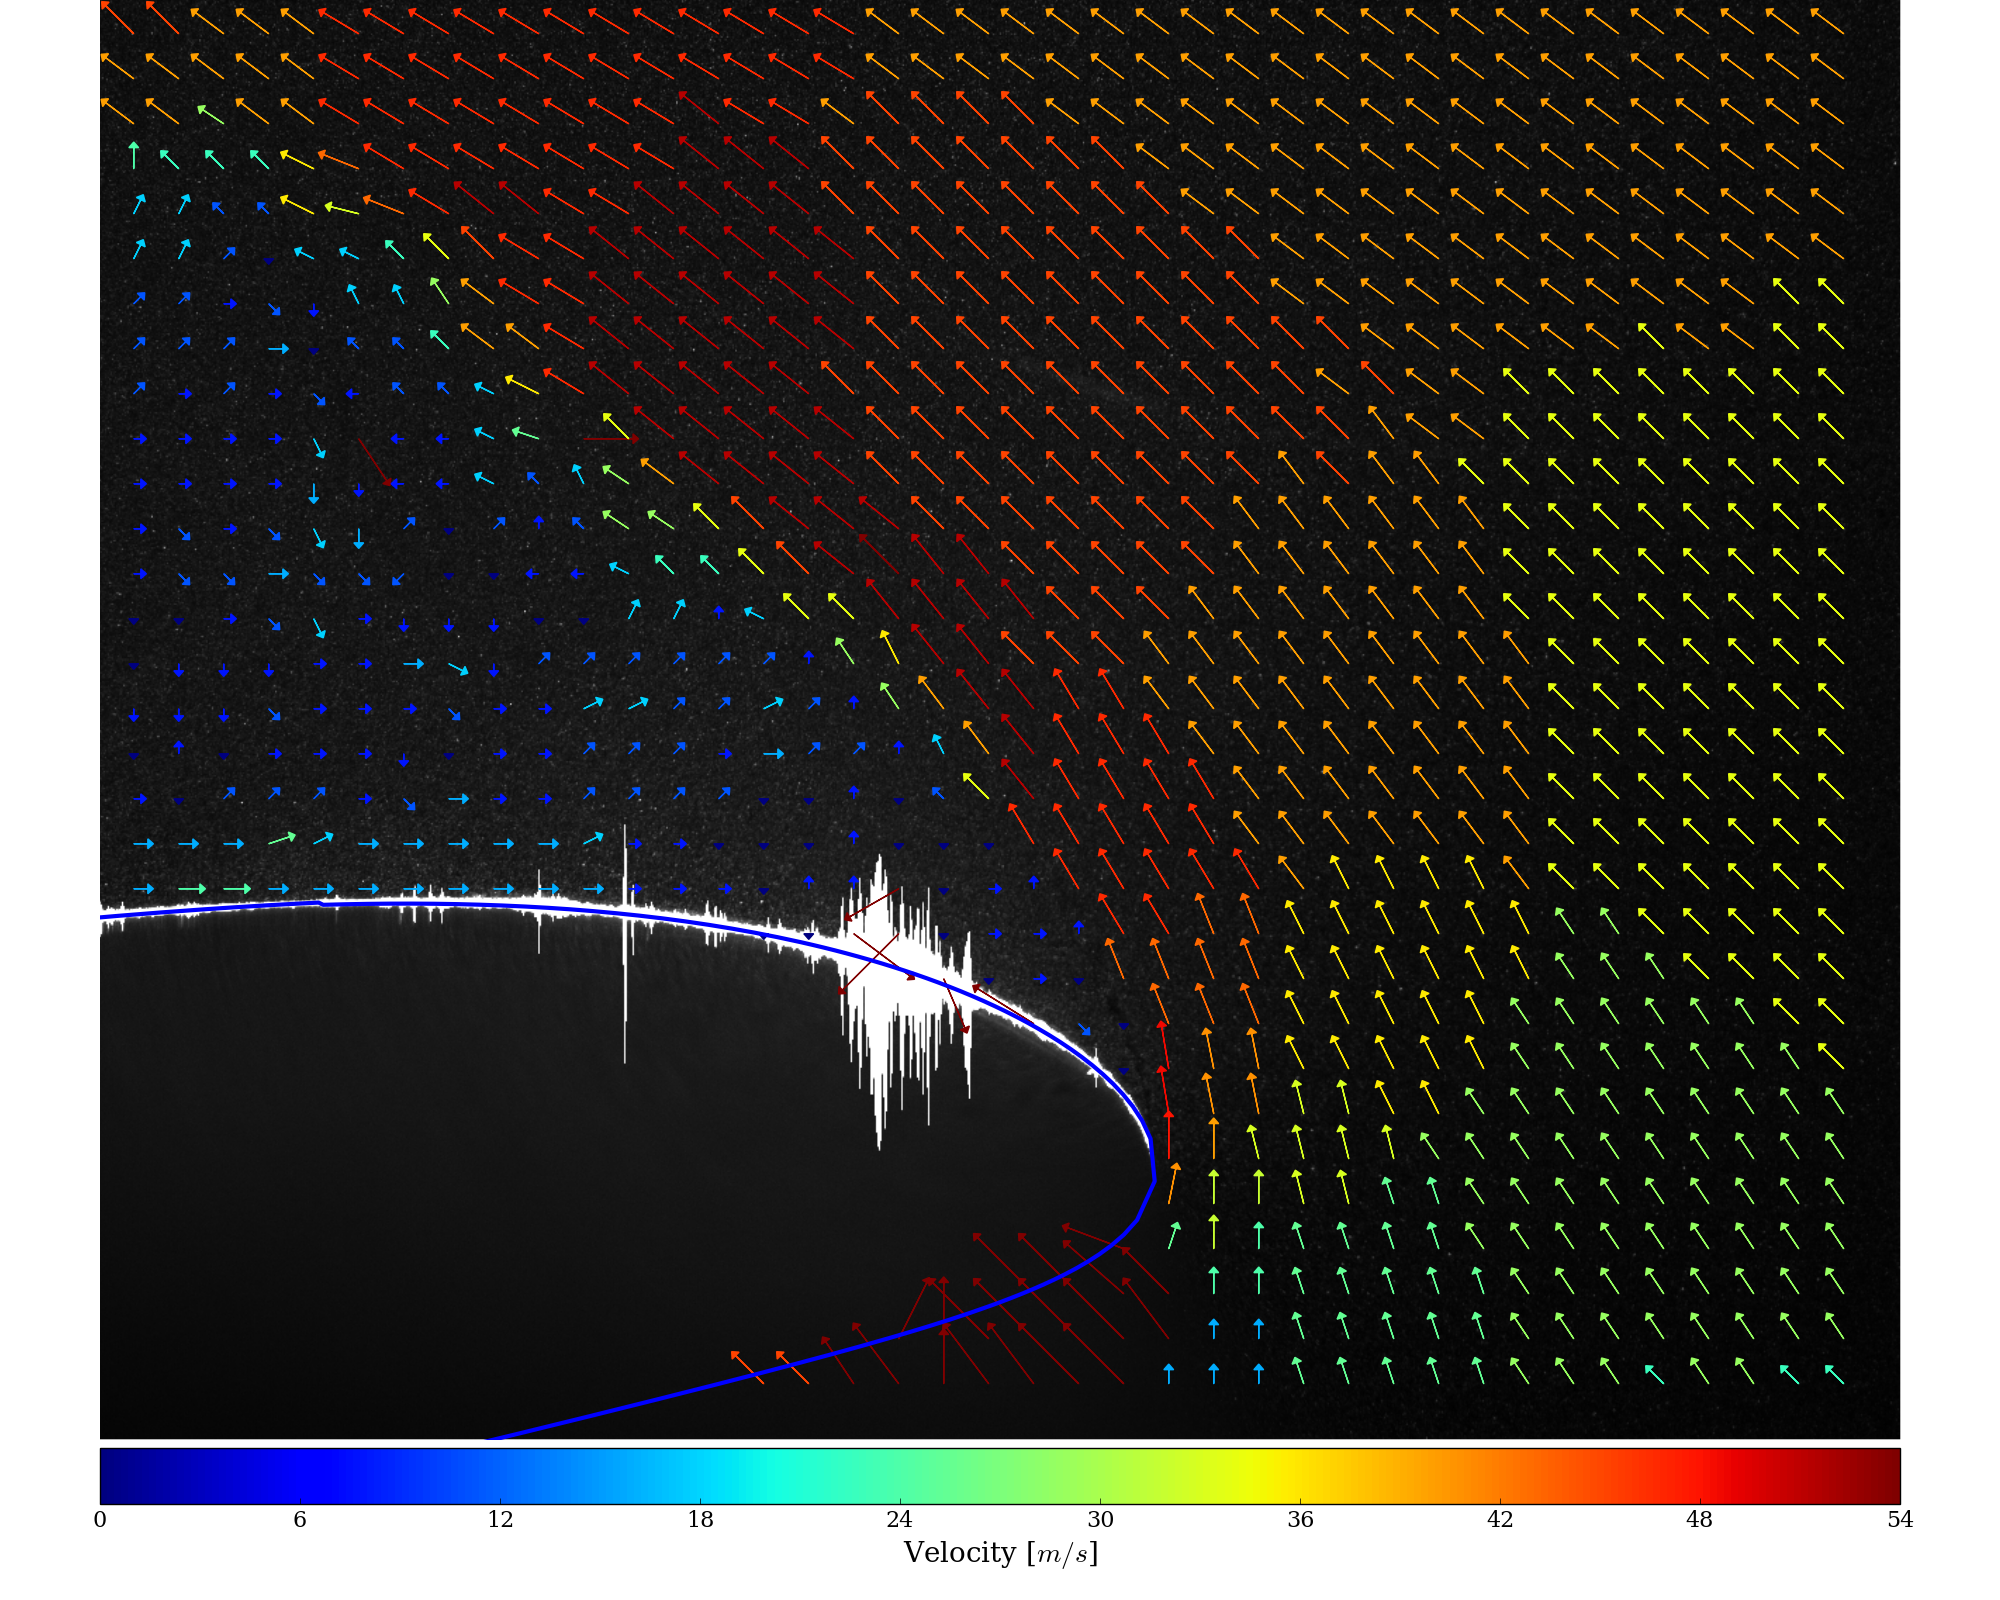
\includegraphics[width=0.48\textwidth]{images/ssd_CM_32_orig.png}}
	\caption{PIV con correlazione SSD}
	\label{fig:ssd}
\end{figure}

\subsection{NCC con interpolazione sub-pixel}

La correlazione secondo l'eq.\ref{eq:ncc}, unitamente all'interpolazione secondo l'eq.\ref{eq:pf}, porta a risultati soddisfacenti, sia considerando finestre di interrogazione da $32px$ (figura \ref{fig:ncc:b}), in cui sono praticamente assenti correlazioni spurie, sia considerando finestre di interrogazione da $16px$ (figura \ref{fig:ncc:a}), in cui il campo di velocità è risolto molto bene, ad eccezione di pochi punti probabilmente spuri nello strato limite e la zona dell'intradosso.

\begin{figure}[ht]
	\centering
	\subfigure[PIV con NCC - finestra 16px\label{fig:ncc:a}]
	{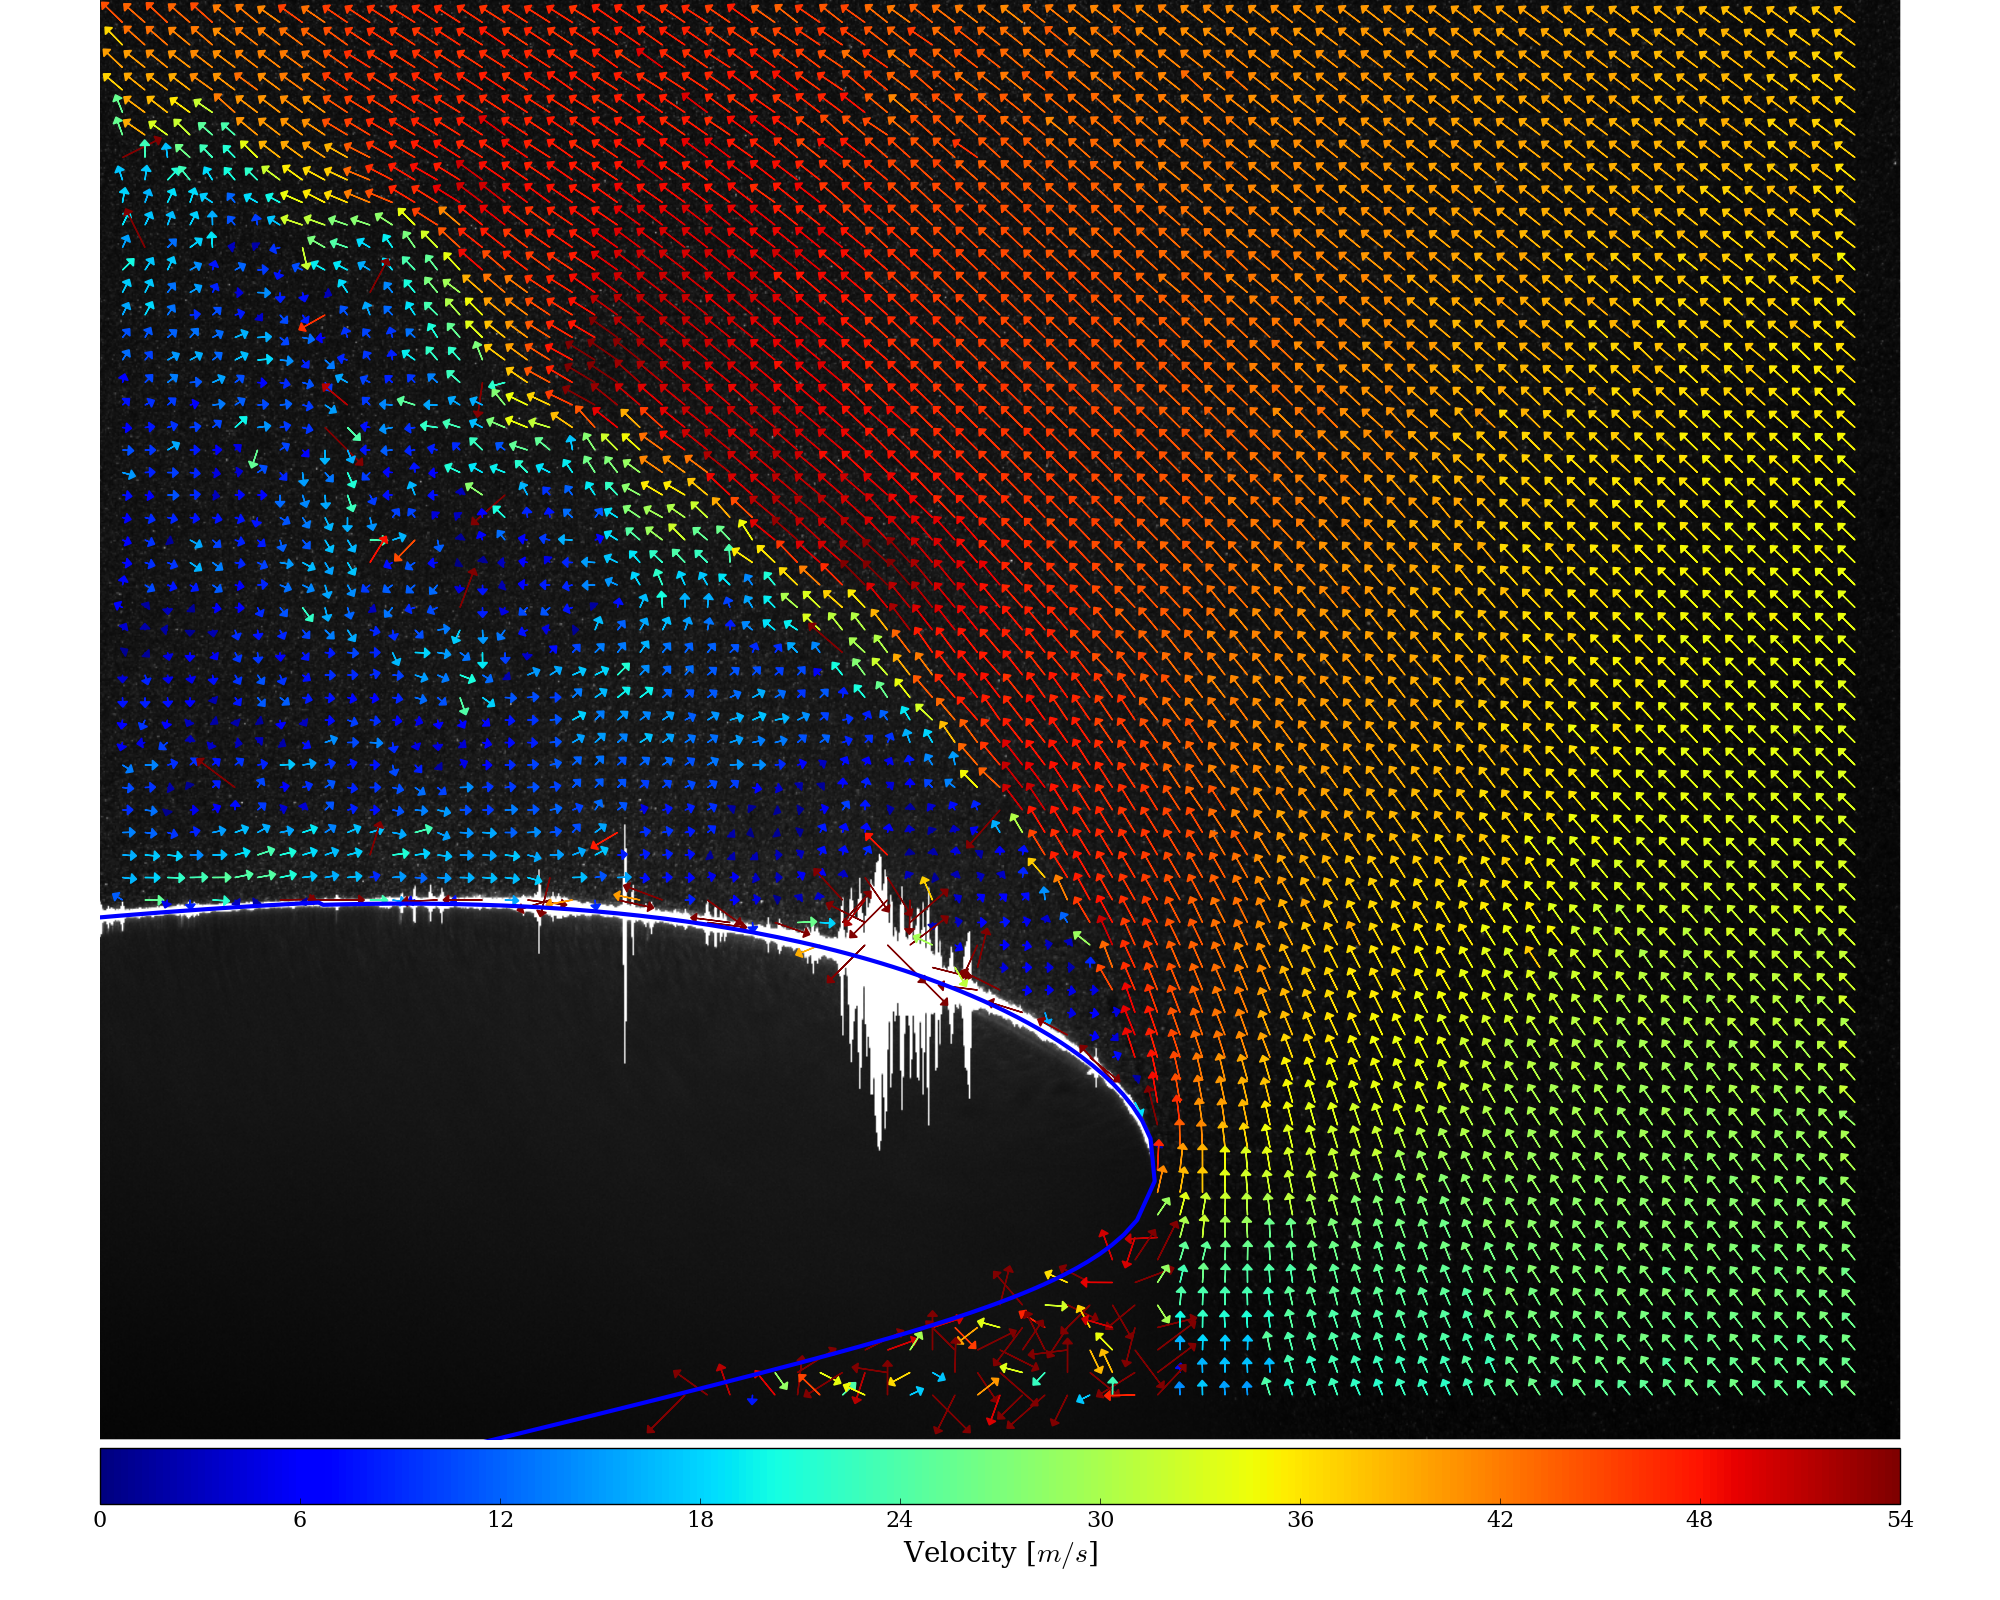
\includegraphics[width=0.48\textwidth]{images/norm_CM_16_orig.png}}
	%\hspace{0.3\textwidth}
	\subfigure[PIV con NCC - finestra 32px\label{fig:ncc:b}]
	{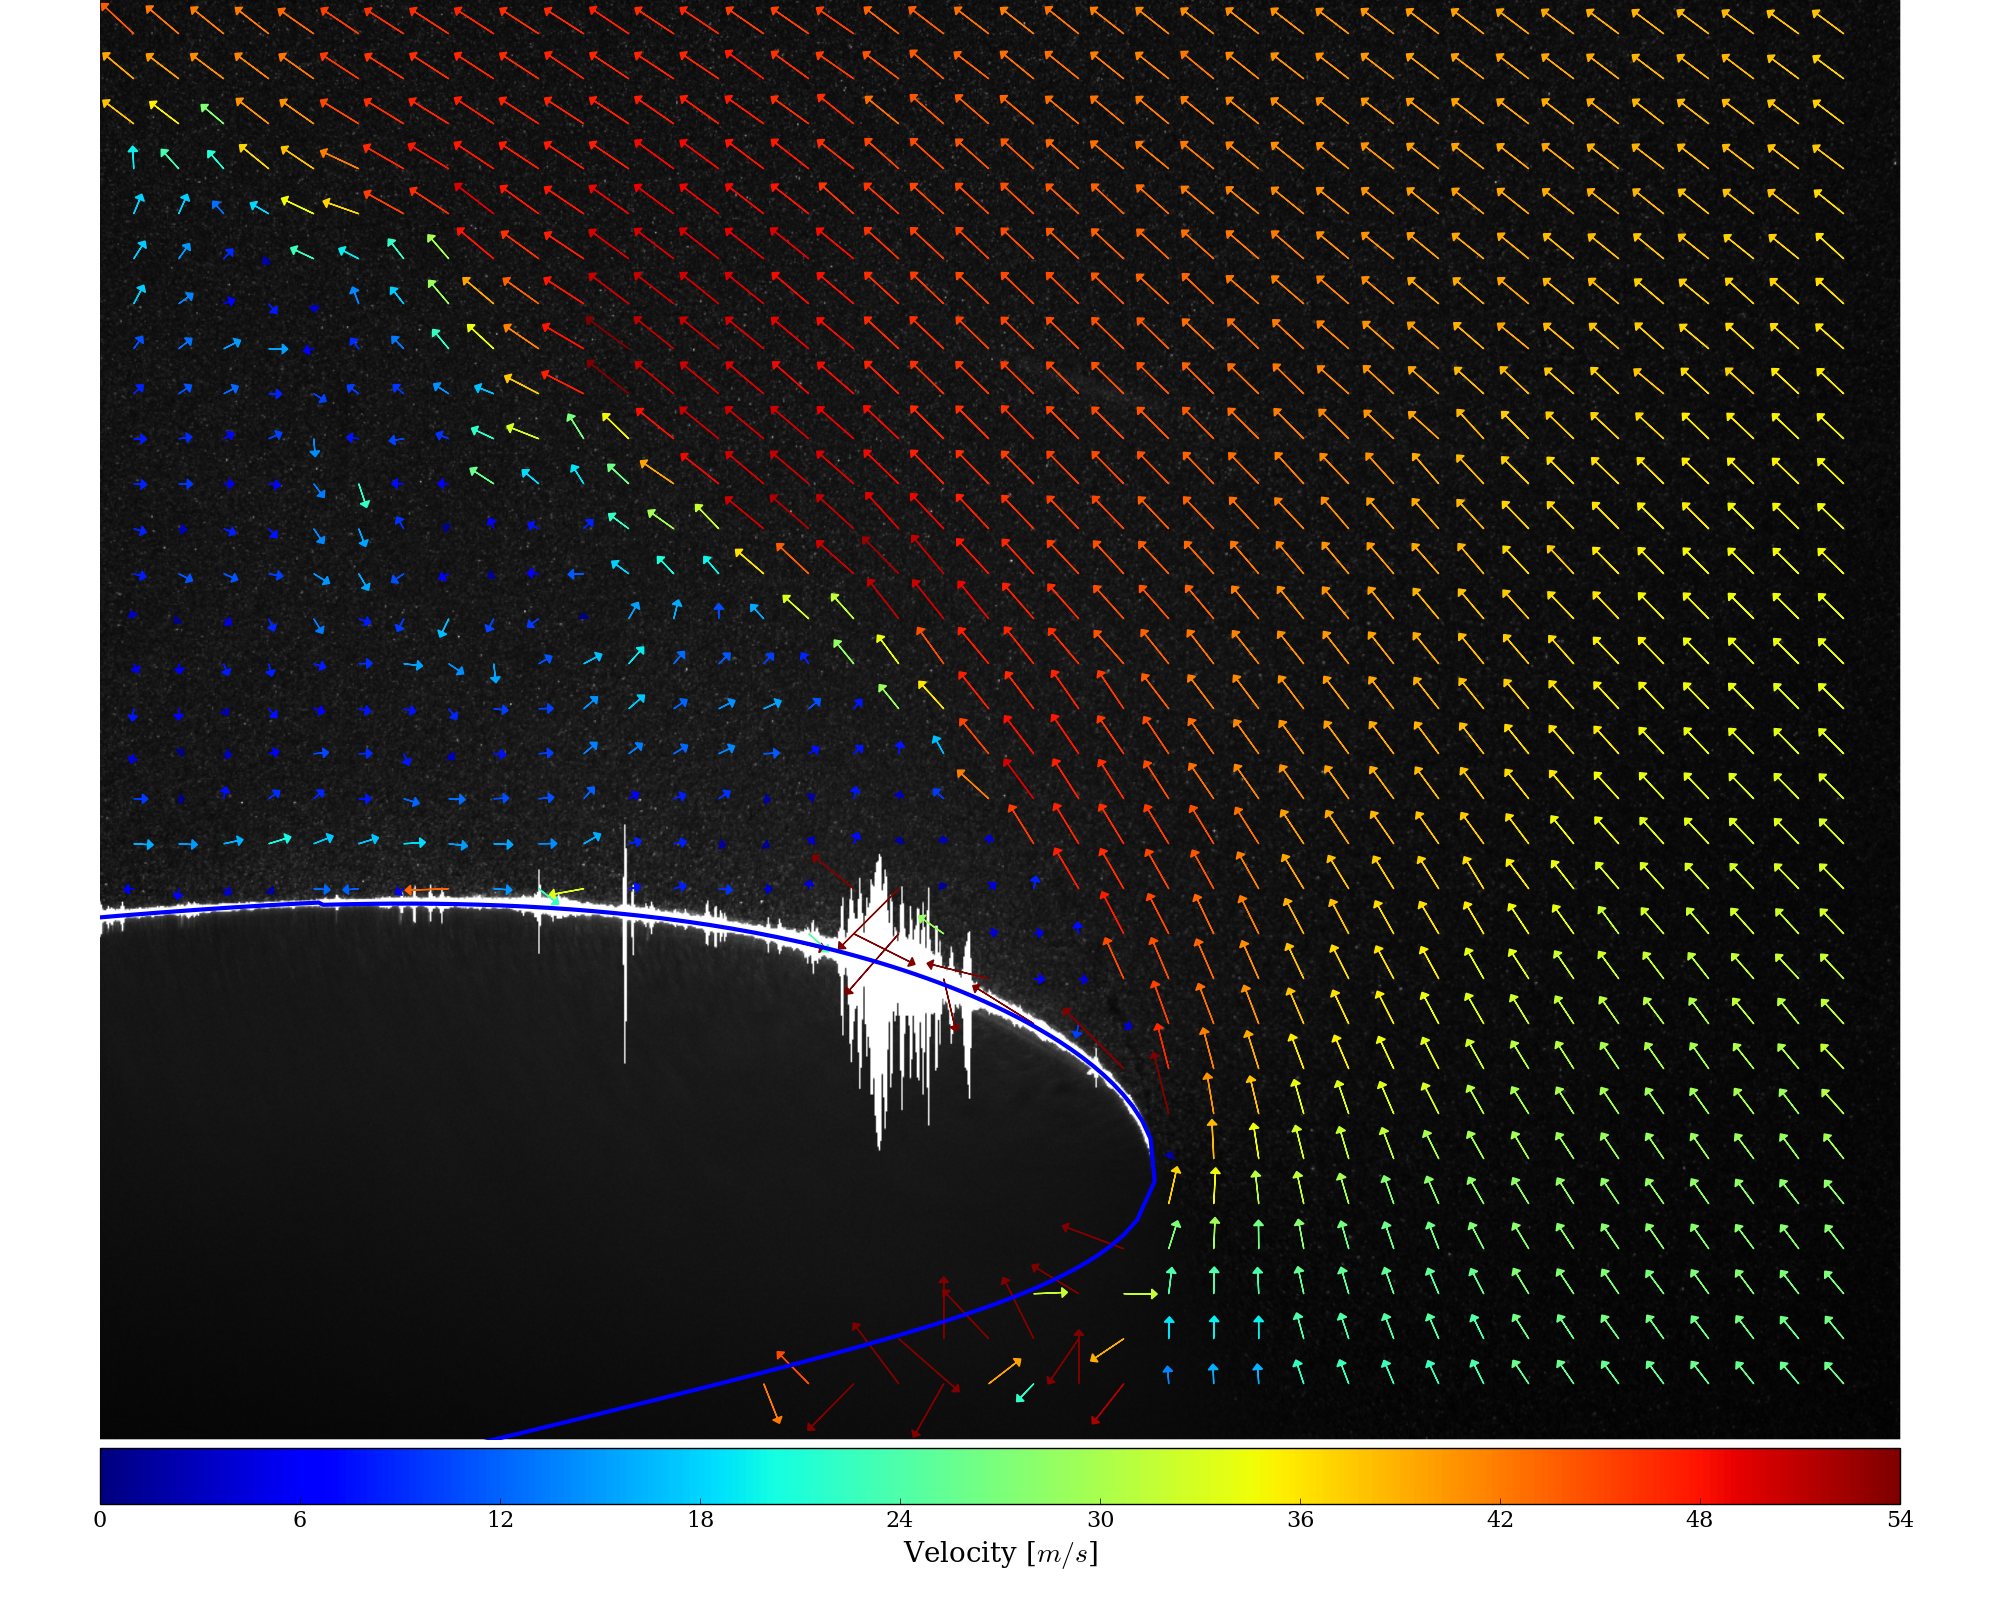
\includegraphics[width=0.48\textwidth]{images/norm_CM_32_orig.png}}
	\caption{PIV con correlazione NCC}
	\label{fig:ncc}
\end{figure}


\subsection{DFT}

Seguendo l'esempio descritto in \cite{scikit}, è stata implementata la PIV utilizzando funzioni di libreria che consentono di determinare lo \textit{shift} tra due immagini tramite \textit{trasformata di Fourier} con upsampling per ottenere una precisione sub-pixel. Utilizzando una finestra di interrogazione da $32px$ (figura \ref{fig:dft:b}) il risultato è sostanzialmente identico a \textbf{NCC}. Una finestra di interrogazione da $16px$  (figura \ref{fig:dft:a}) comporta un elevato numero di vettori spuri nella regione al di fuori dello strato limite.

\begin{figure}[ht]
	\centering
	\subfigure[PIV con DFT - finestra 16px\label{fig:dft:a}]
	{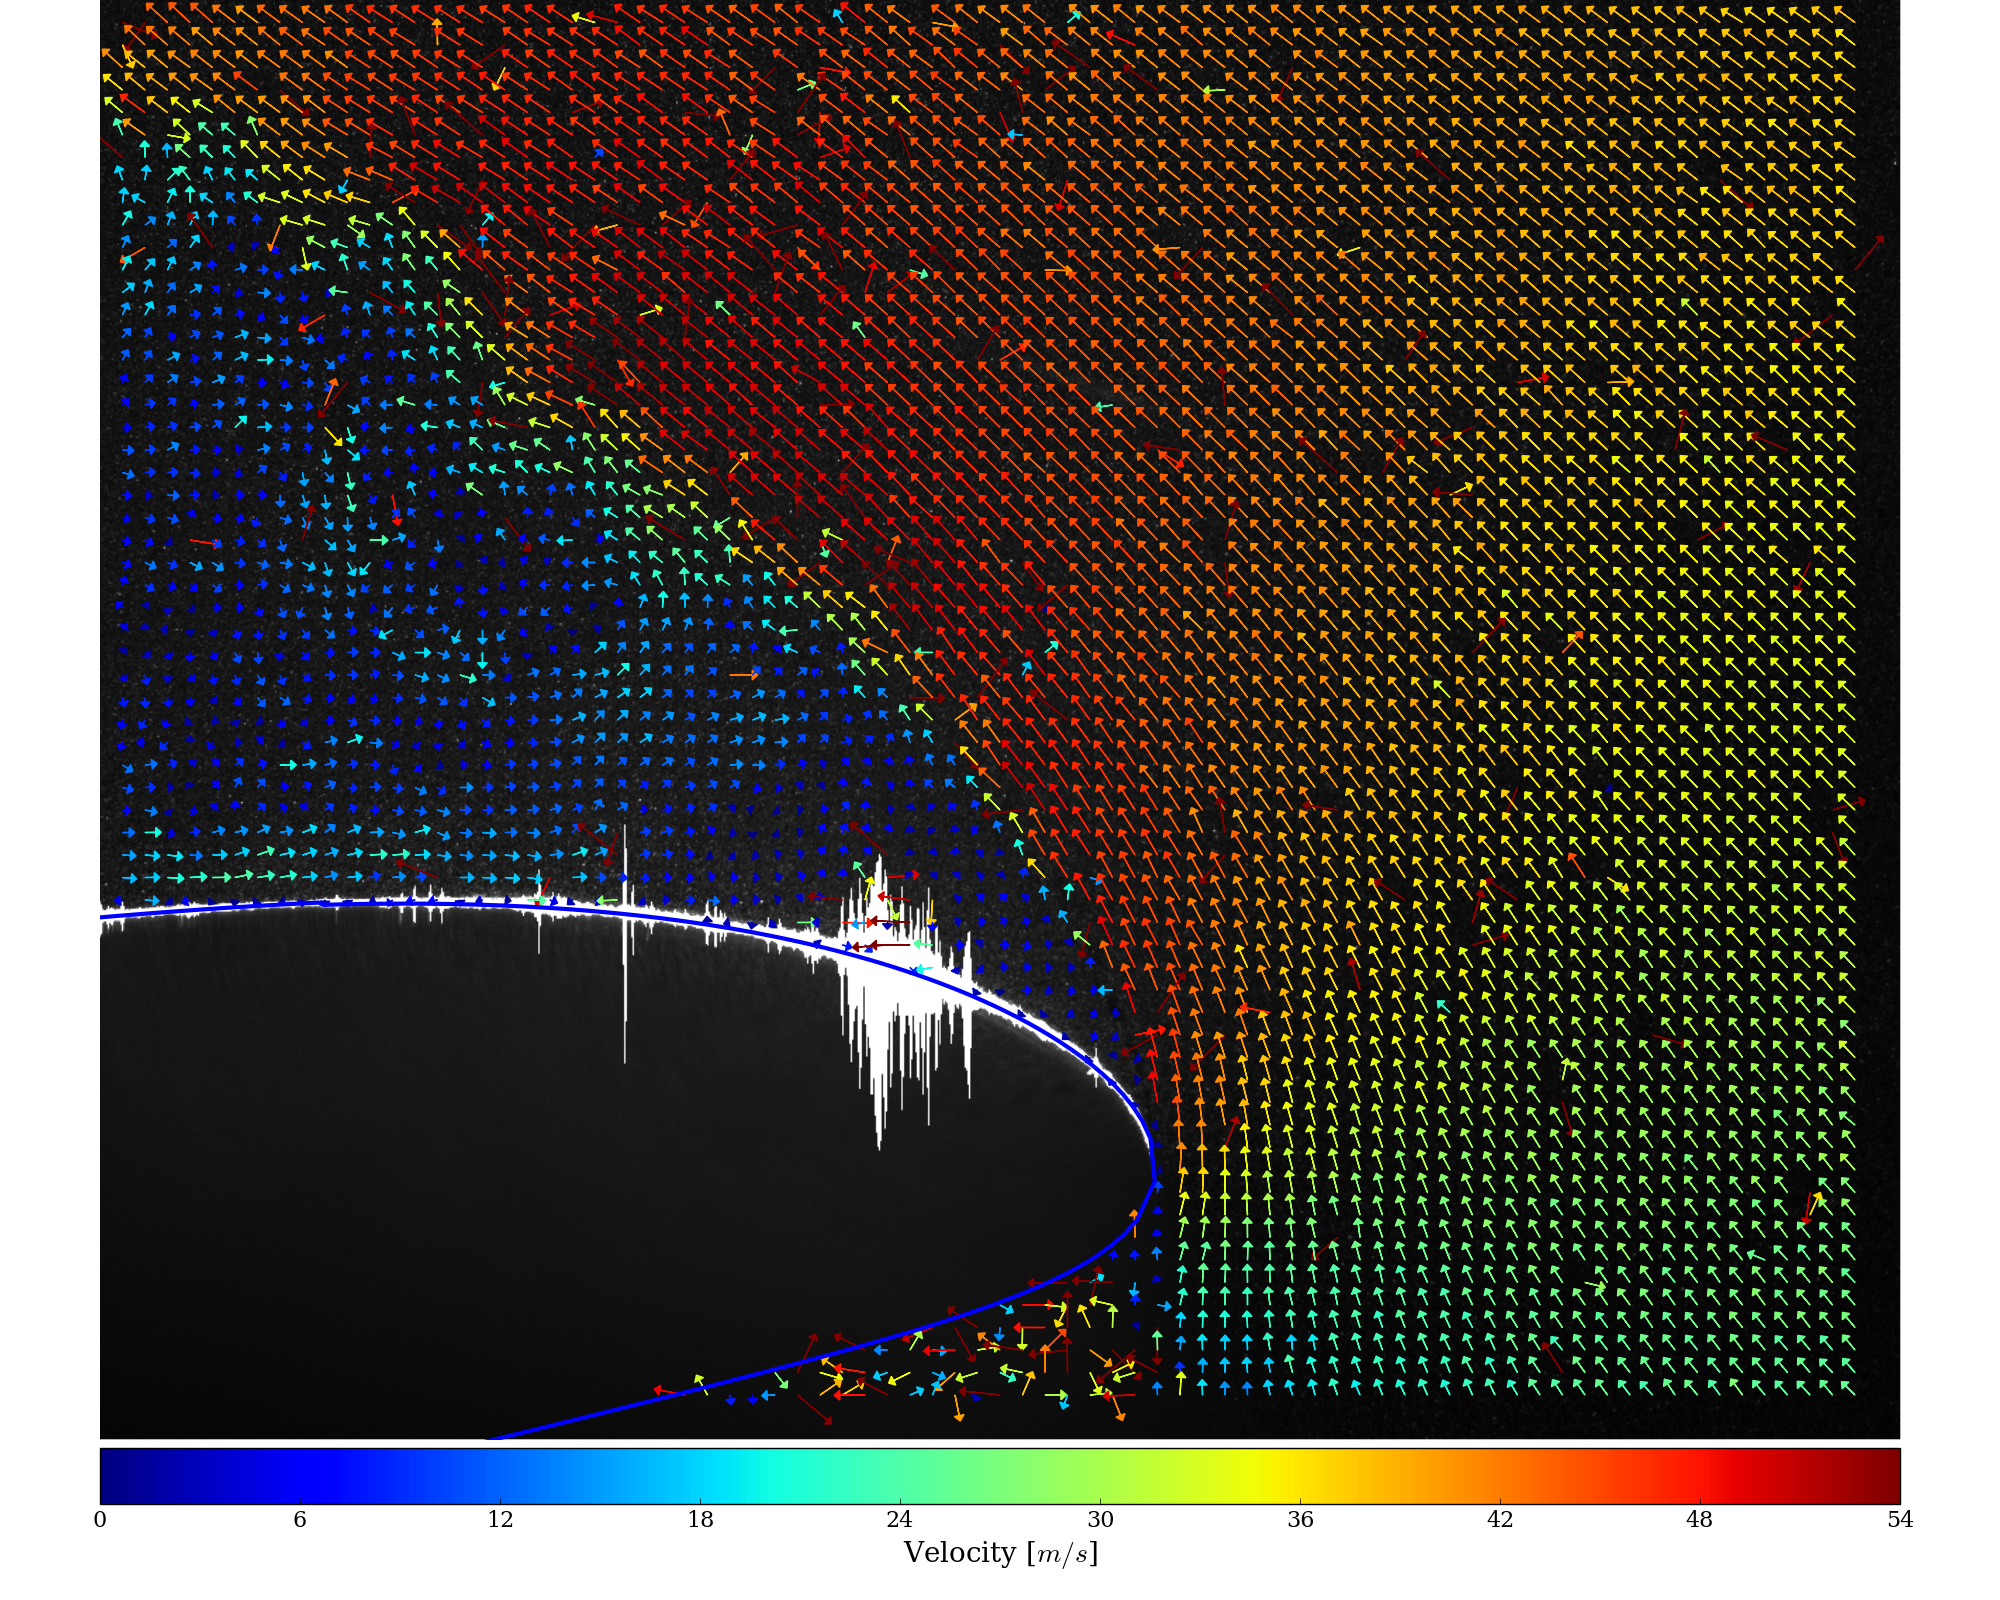
\includegraphics[width=0.48\textwidth]{images/scikit_CM_16_orig.png}}
	%\hspace{0.3\textwidth}
	\subfigure[PIV con DFT - finestra 32px\label{fig:dft:b}]
	{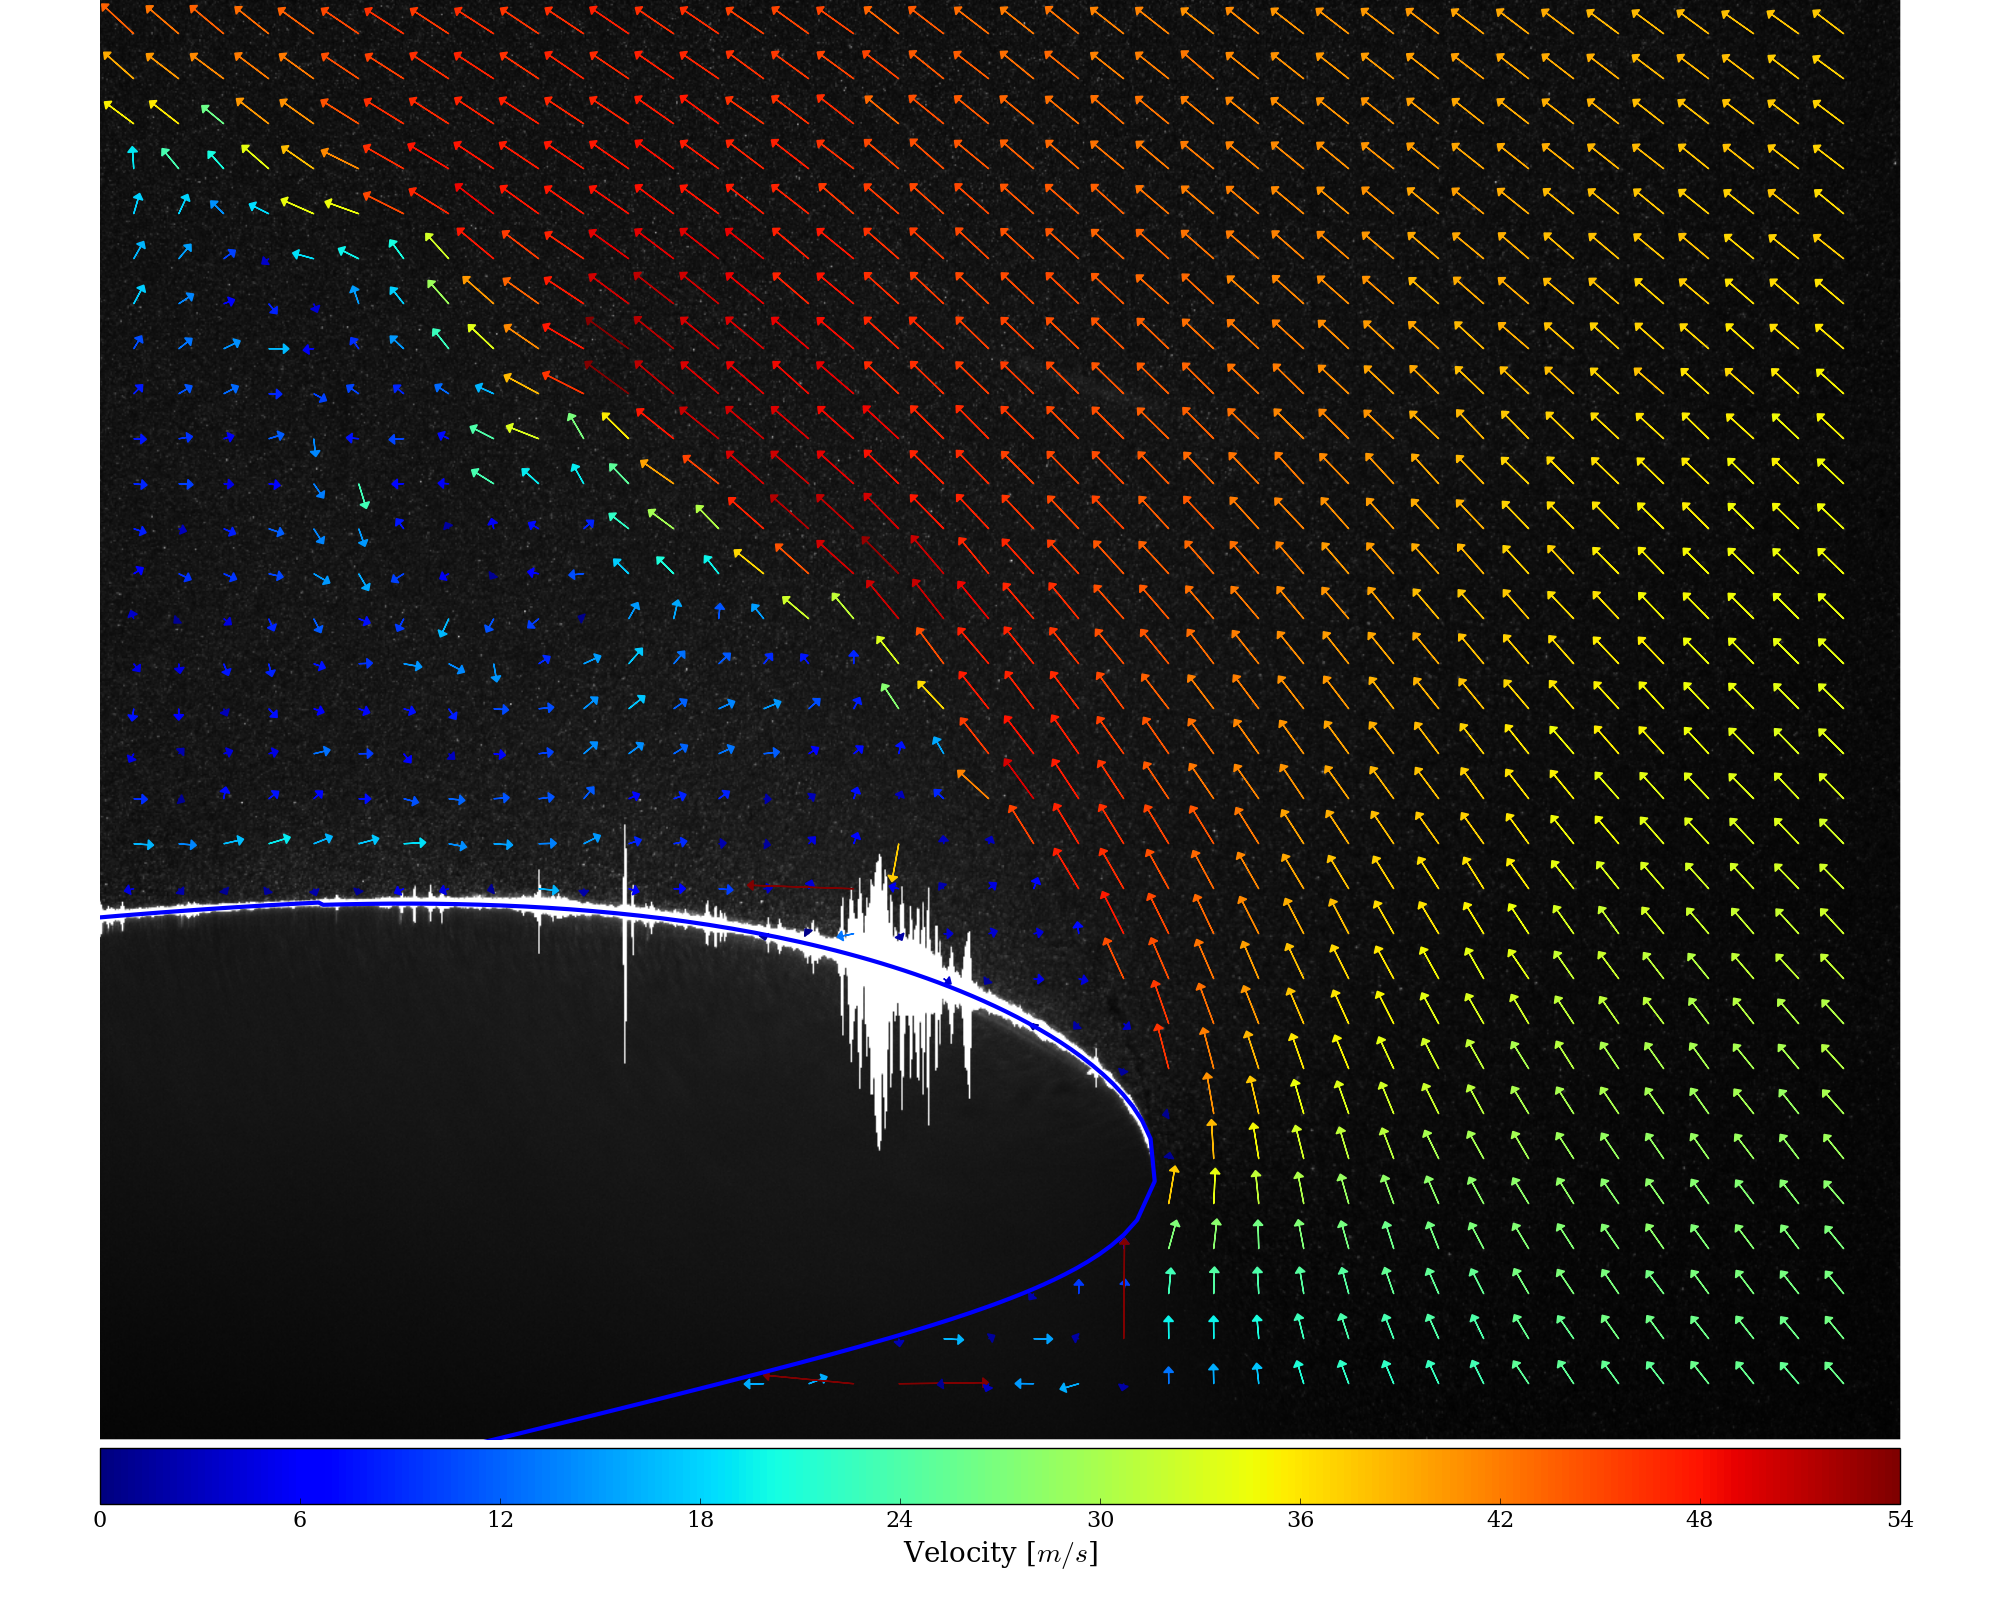
\includegraphics[width=0.48\textwidth]{images/scikit_CM_32_orig.png}}
	\caption{PIV con correlazione DFT}
	\label{fig:dft}
\end{figure}


\section{Post-Processing}

Una volta determinato il campo di spostamenti in pixel è necessario eseguire alcune operazioni di \textit{post-processing}.

\paragraph{Conversione}: è necessario passare dagli spostamenti in pixel al valore di velocità, secondo la formula:

\begin{equation}
v \left[m/s\right] = \sqrt{\Delta x^2 + \Delta y^2}px \cdot \frac{1}{10\cdot10^{-6}s} \cdot \frac{0.082m}{1024px}
\label{eq:conv}
\end{equation}

Il fattore di conversione di eq. \ref{eq:conv} è stato utilizzato per tutte le figure presentate.

\paragraph{Dati spuri}: tutti i dati di velocità spuri possono teoricamente essere sostituiti utilizzando i valori degli 8 elementi vicini, se ritenuti corretti. Il procedimento richiederebbe di identificare vettori molto diversi dai confinanti in termini di modulo e direzione e sostituirli con opportune medie. Poiché la miglior correlazione ottenuta (\textbf{NCC}) non presenta un numero sufficiente di dati palesemente spuri, si è deciso di non implementare questa operazione.

\section{Codice di calcolo}

Il linguaggio utilizzato per effettuare l'analisi è \textit{Python} ed il codice implementato è visibile all'indirizzo \url{https://github.com/Ccaccia73/FS_report} nella cartella \textsc{code}.\\
Un esempio della sequenza di oerazioni è visibile (non eseguibile) all'indirizzo \url{http://nbviewer.jupyter.org/github/ccaccia73/FS_report/blob/master/code/PIV.ipynb}


\newpage

\section{Confronto con OpenPIV}

OpenPIV è un pacchetto software (\url{http://www.openpiv.net/}) open-source per l'analisi ed il post-processing di immagini PIV. \`{E} implementato in diversi linguaggi e fornisce diverse funzionalità per il filtraggio e l'analisi. Come ulteriore analisi e per valutare la qualità dei risultati ottenuti, sono state eseguite alcune analisi con la versione del programma in \textsc{C++}.  









\newpage


\section{Figure Aggiuntive}

\begin{figure}[h]
	\centering
	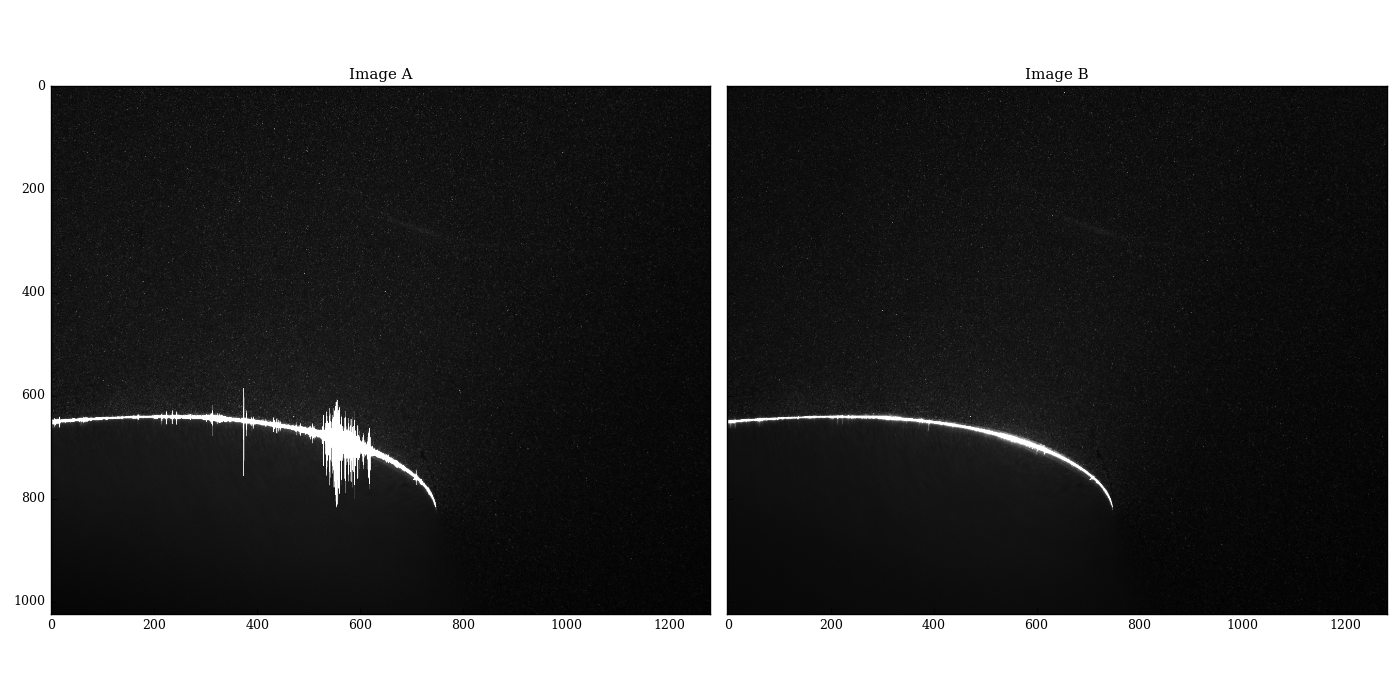
\includegraphics[width=1\textwidth]{images/raw_images.png}
	\caption{Immagini originali}
	\label{fig:img}
\end{figure}


 \begin{figure}[h]
 	\centering
 	\subfigure[PIV con Correlazione - finestra 32px]
 	{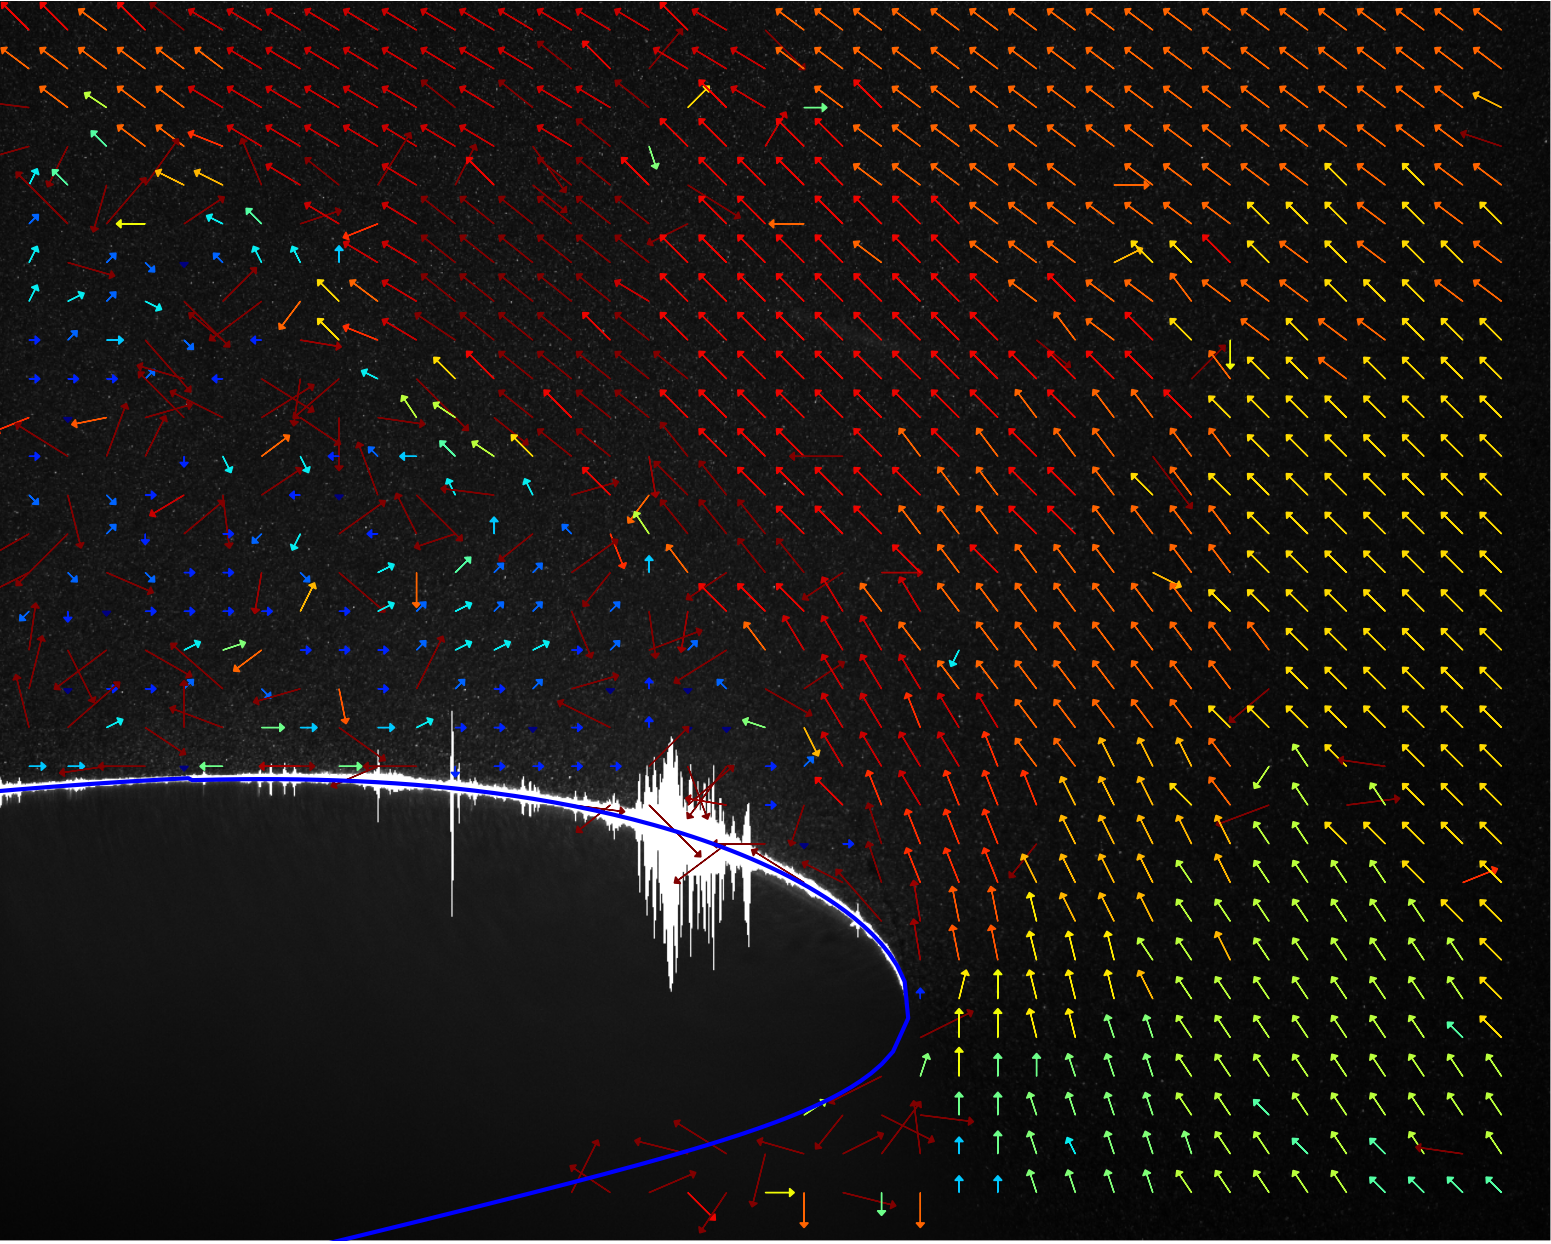
\includegraphics[width=0.48\textwidth]{images/norm_32_filt.png}}
 	%\hspace{0.3\textwidth}
 	\subfigure[PIV con DFT - finestra 32px]
 	{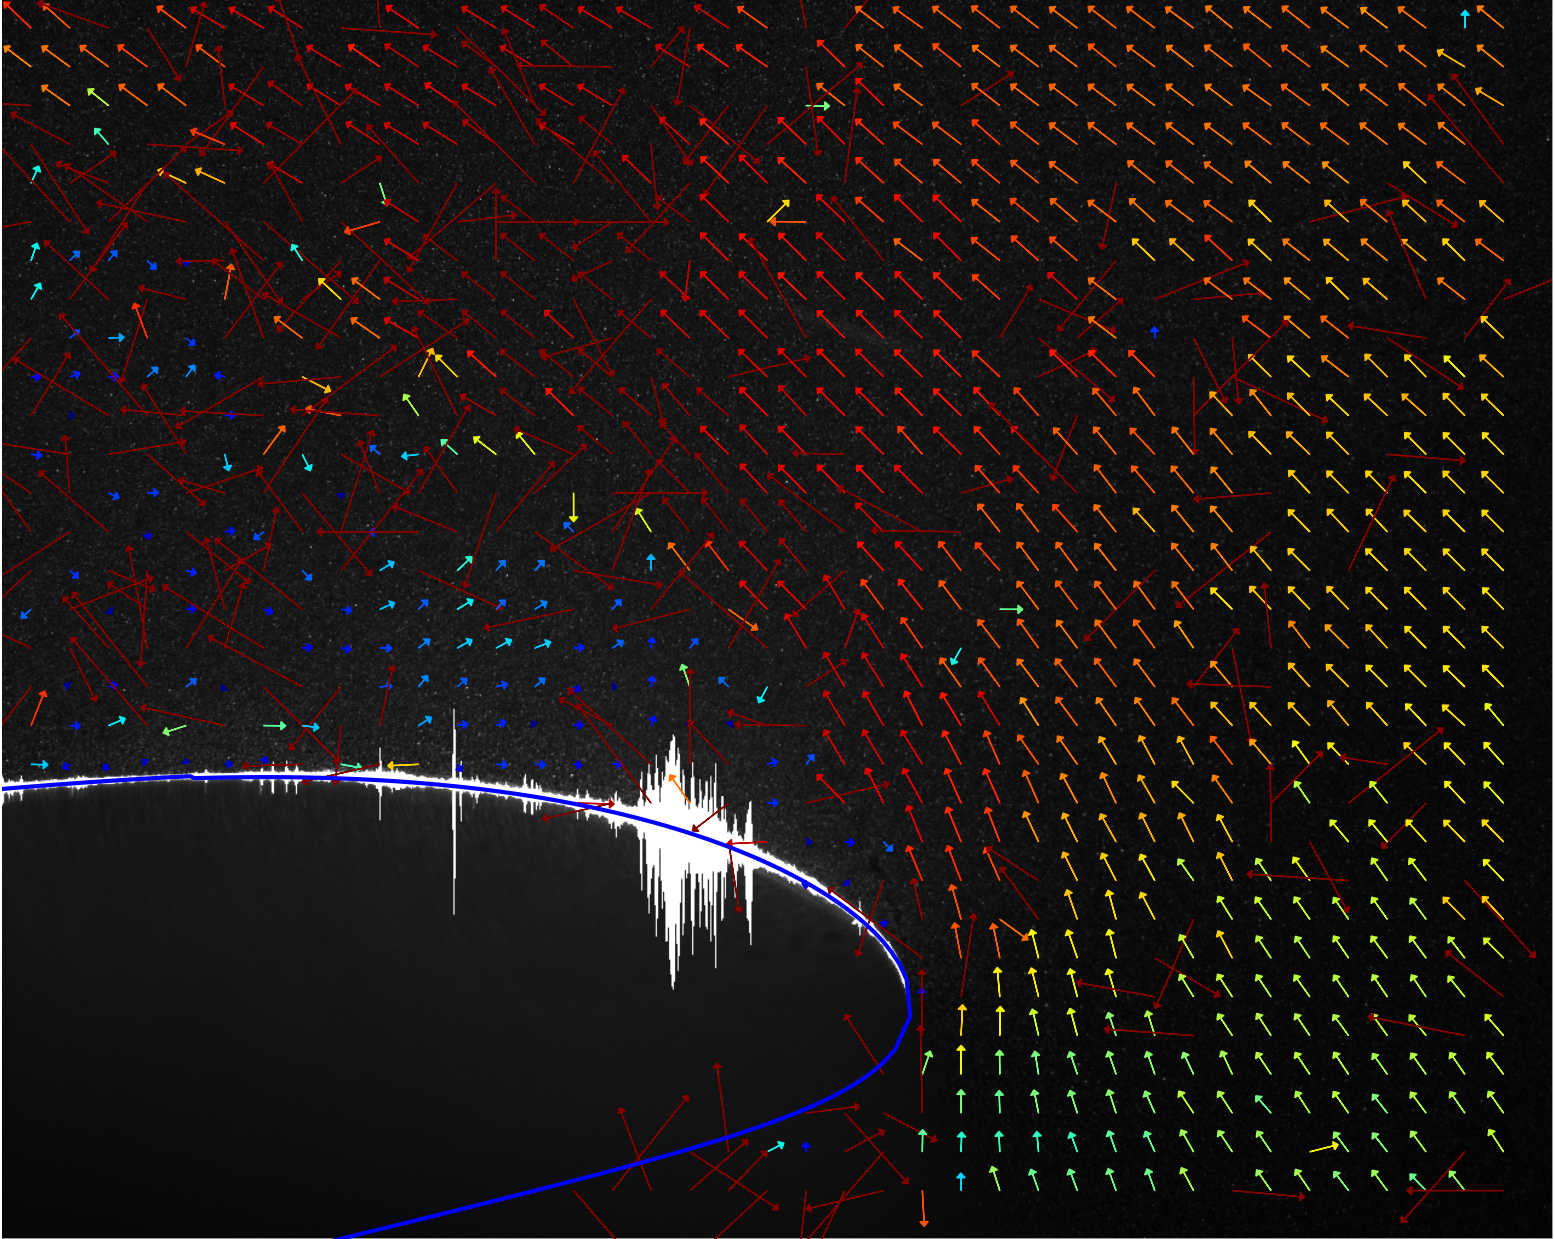
\includegraphics[width=0.48\textwidth]{images/scikit_32_filt.png}}
 	\caption{PIV su immagini filtrate}
 	\label{fig:filt_piv}
 \end{figure}

\begin{figure}[h]
	\centering
	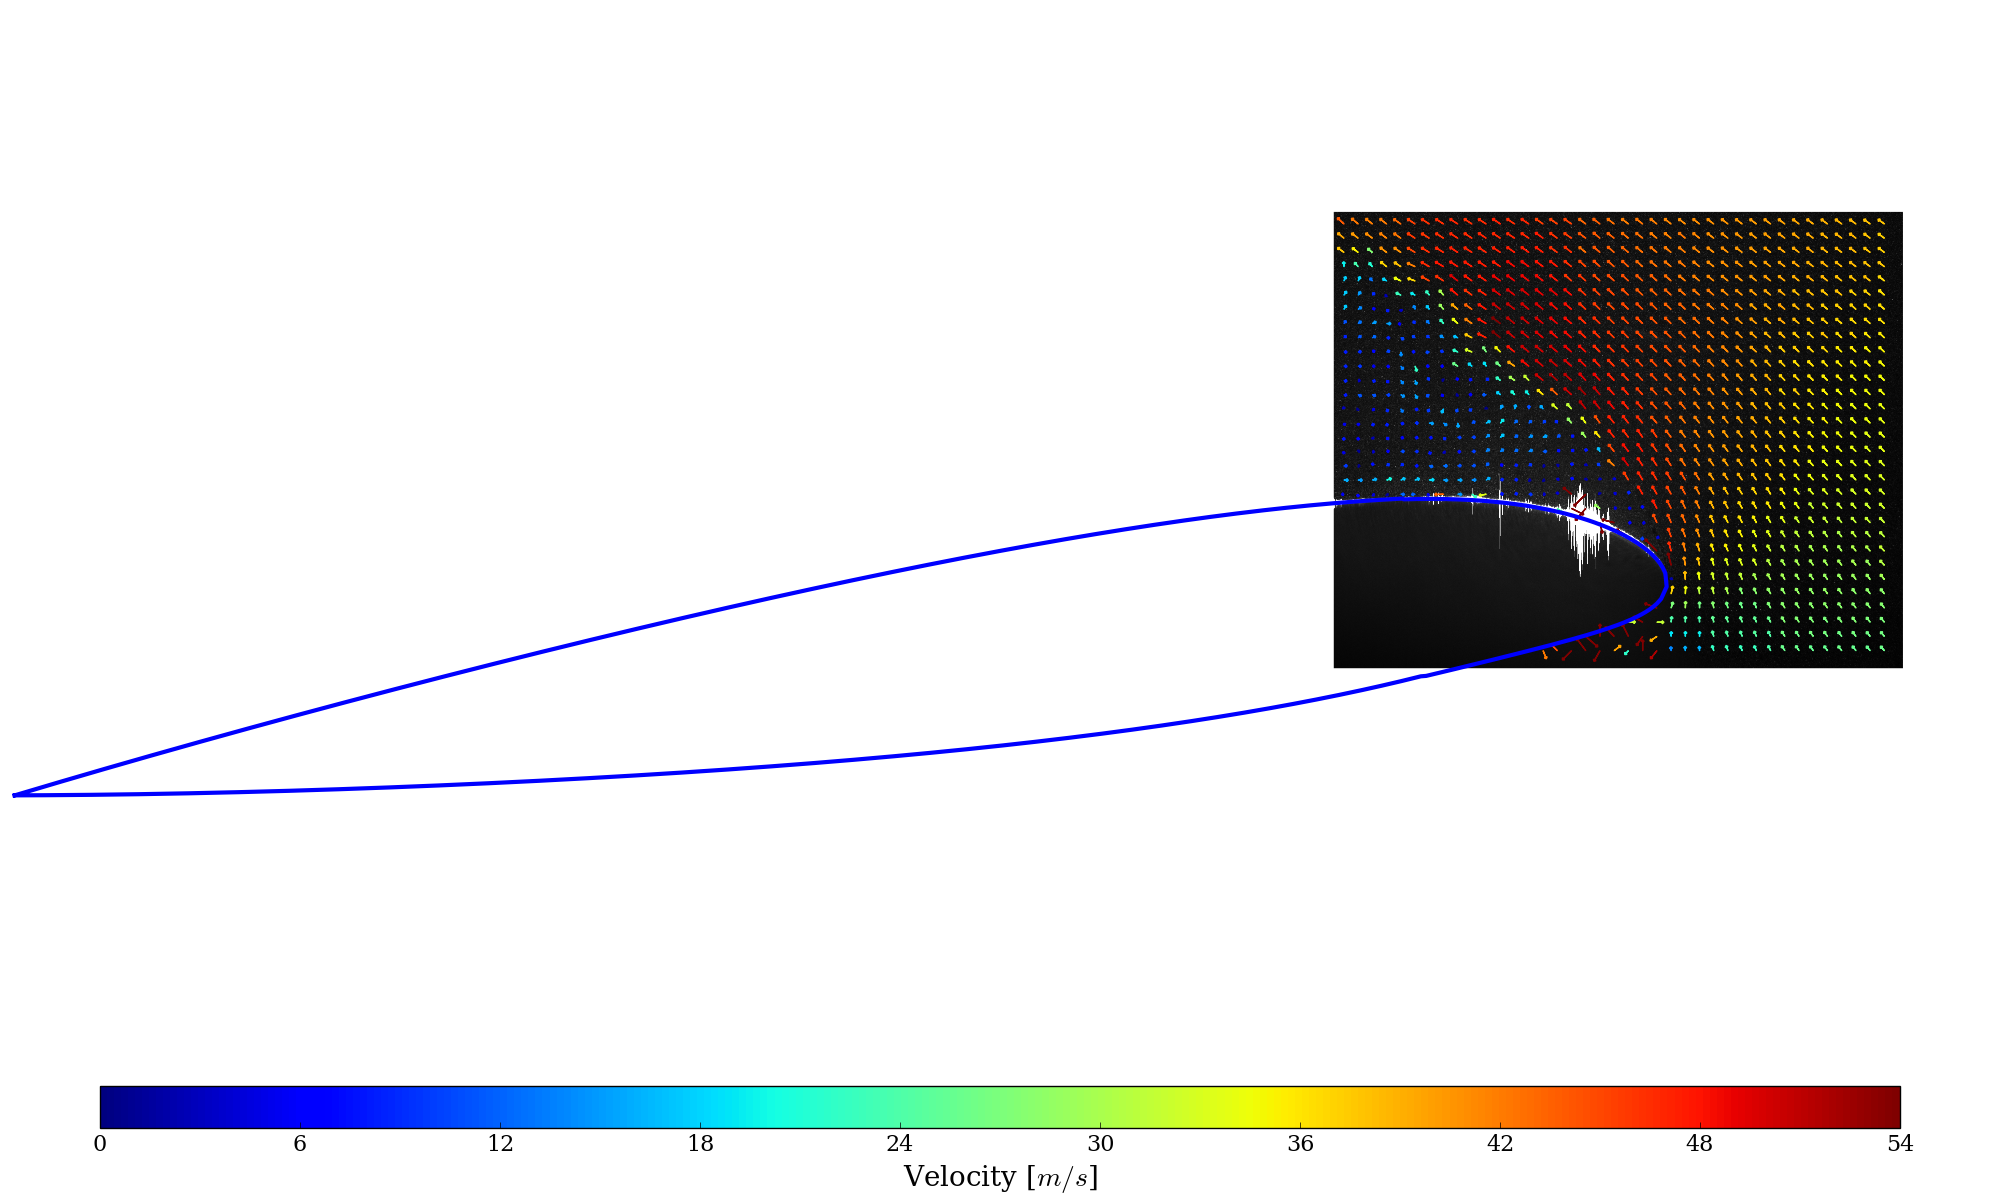
\includegraphics[width=1\textwidth]{images/All_norm_CM_32_orig.png}
	\caption{Profilo alare e regione PIV}
	\label{fig:airfoil}
\end{figure}

\newpage

\begin{thebibliography}{9}
\bibitem{mmaxf}
Deen, Niels G., et al. "On image pre-processing for PIV of single-and two-phase flows over reflecting objects." Experiments in fluids 49.2 (2010): 525-530.

\bibitem{corrCV}OpenCV object Detection, \url{http://docs.opencv.org/2.4/modules/imgproc/doc/object_detection.html?highlight=matchtemplate#matchtemplate}

\bibitem{imcorr}
Pan, Bing, and Kai Li. "A fast digital image correlation method for deformation measurement." Optics and Lasers in Engineering 49.7 (2011): 841-847.

\bibitem{ncc}
Zhao, Feng, Qingming Huang, and Wen Gao. "Image matching by normalized cross-correlation." Acoustics, Speech and Signal Processing, 2006. ICASSP 2006 Proceedings. 2006 IEEE International Conference on. Vol. 2. IEEE, 2006.

\bibitem{spim}
Westerweel, Jerry. "Digital particle image velocimetry." Delft University (1993): 75-78.

\bibitem{spdft}
Guizar-Sicairos, Manuel, Samuel T. Thurman, and James R. Fienup. "Efficient subpixel image registration algorithms." Optics letters 33.2 (2008): 156-158.


\bibitem{scikit}Scikit-Image cross-correlation,
\url{http://scikit-image.org/docs/dev/auto_examples/transform/plot_register_translation.html}

\bibitem{openpiv}
Liberzon, A., R. Gurka, and Z. Taylor. "Openpiv home page." (2009).

\end{thebibliography}
\end{document}